Consider the following snippet. It represents the encoding of the negation of modus ponens
($\neg (p \rightarrow ((p \rightarrow q) \rightarrow q))$) as an SMT problem using SMT-LIB~\cite{smtlib},
a standardized syntax for representing SMT problems:

\begin{figure}[h]
\begin{minted}{smtlib2.py -x}
  (set-logic QF_UF)
  (declare-const p Bool)
  (declare-const q Bool)
  (assert (not (=> p (=> (=> p q) q))))
\end{minted}
\caption{SMT-LIB script representing the negation of modus ponens.}\label{negModusPonens}
\end{figure}

We will illustrate the process of reconstructing proofs of cvc5 via certified transformations
in Lean through this example. Feeding this script to cvc5 yields the result ``unsat'', as expected.
The proof produced by the solver is shown in Figure~\ref{fig:cvc5-proof}\footnote{This was produced with the proof visualizer tool, available at: \url{https://ufmg-smite.github.io/proof-visualizer/}} and is an instance of the resolution tree introduced in Section~\ref{sec:pcBool}.
Each node is a formula that is either the one from the input (\texttt{not (=> p (=> (=> p q) q))}) or was derived by applying some
rule to other nodes. An edge from some node $u$ to other node $v$ indicates that
$u$ was used to derive $v$.
In addition to the resolution rule (in purple and green), there are also rules for conjunctive normal form transformations (yellow)\footnote{The rules in the figure are in the internal calculus of cvc5, which is documented in \url{https://cvc5.github.io/docs/latest/proofs/proof_rules.html}}. Note that all leaves (in blue) correspond to the input formula.

\makeatletter
\setlength{\@fptop}{0pt}
\makeatother

\begin{figure}[t!]
  \centering
  \scalebox{0.45}{%
    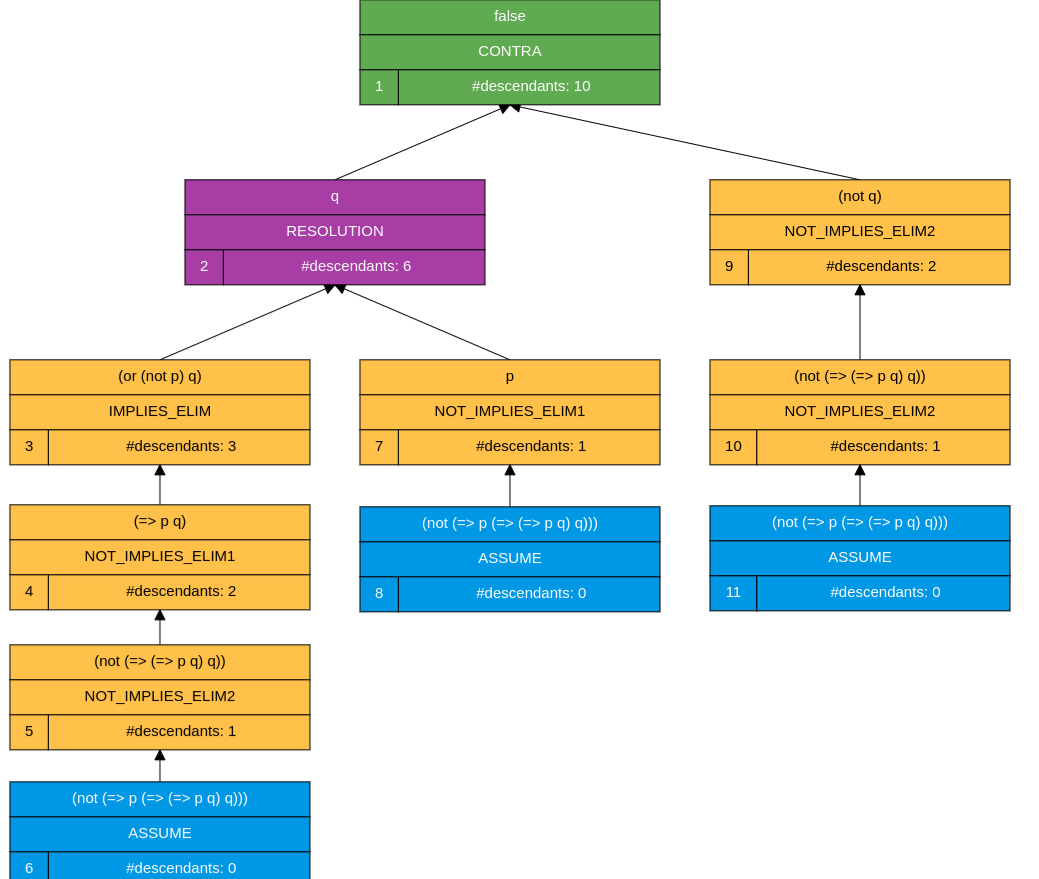
\includegraphics[scale=0.9]{img/mp_cvc5_proof.png}}
  \caption{A cvc5 proof for the validity of Modus Ponens.}
  \label{fig:cvc5-proof}
\end{figure}

The encoding of this proof into Lean requires representing the terms that appear
in it, i.e.\ the formulas built with $p$ and $q$, as well as the rules.
%
This representation uses a \emph{deep embedding} of the proof calculus of cvc5 into
Lean,
which is done via a \texttt{term} type that models terms and formulas from MSFOL.
The \texttt{const} constructor of this type can be used to define symbols,
which are parameterized by an identifier (a natural number) and a \texttt{sort}
(another type for enconding MSFOL sorts).
%
For example, in the formula for modus ponens, \texttt{p} and \texttt{q} are
free variables, which can be treated as constants while defining the problem in Lean.
The following snippet shows their declaration using the \texttt{term} type:

\begin{minted}{lean}
  def p: term := const 1 boolSort
  def q: term := const 2 boolSort
\end{minted}

The identifiers \texttt{1} and \texttt{2} are arbitrary, with only the
requirement that they are unique.

With these terms and using the functions \texttt{implies} and
\texttt{not} defined in the deep embedding corresponding to the MSFOL symbols
$\rightarrow$ and $\neg$, we encode the formula used in the
query:

\begin{minted}{lean}
  def modusPonensEmbed: term := implies p (implies (implies p q) q)
  def notModusPonensEmbed: term := not modusPonensEmbed
\end{minted}


\subsection{The Boolean fragment}

We will now implement a function that lifts embedded terms to the corresponding
native Lean terms, so that we can prove facts about them using Lean.
Initially, we will limit ourselves to the fragment of MSFOL that
deals with Boolean values\footnote{The Boolean fragment of the
\emph{Core} theory in SMT-LIB, as defined in
\url{http://smtlib.cs.uiowa.edu/theories-Core.shtml}}. Once
we show how to lift this fragment, we will present a generalization
of our definitions that is able to lift any theory from MSFOL.

While designing this function, one has a
choice regarding which type from Lean to use as a counterpart of the Boolean terms. The two
most suitable alternatives are the \texttt{Prop} and \texttt{Bool} types. The former, as
previously explained, is the type used to model all propositions in the language, while
the latter is the usual type of booleans inhabited by only two values: \texttt{true} and
\texttt{false}. While \texttt{Bool} has a simpler structure and potentially would not
require the \texttt{Classical} module (since it is possible to prove classical statements over Booleans),
the extension to other theories will require, necessarily, the usage of \texttt{Prop}. For instance,
consider the equality operator from MSFOL.\ Its applications will be mapped to applications of an equality operator
in Lean. If we map MSFOL's Booleans to \texttt{Bool}, we have to map these applications to the
Boolean equality, which is only defined over certain types. It is not possible
to apply Boolean equality over functions, for instance. On the other hand, the equality
defined over \texttt{Prop} is more general, in a way that is possible to apply it to any type.

Note that the term we will evaluate can contain free variables. For those, we will need an auxiliary interpretation function assigning concrete values to them.
Free variables are
identified by a \texttt{Nat} (the built-in Lean type for natural numbers), therefore, we can
represent this information as a function from \texttt{Nat} to
\texttt{Prop}:

\begin{minted}{lean}
  def Interpretation := Nat -> Prop
\end{minted}


\begin{figure}[t]
\begin{minted}{lean}
  def evalTerm (I : Interpretation) (t : term) : Prop :=
    match t with
    | term.const   i  _  => I i
    | term.not     t1    => Not (evalTerm I t1)
    | term.and     t1 t2 => And (evalTerm I t1) (evalTerm I t2)
    | term.or      t1 t2 => Or (evalTerm I t1) (evalTerm I t2)
    | term.implies t1 t2 => (evalTerm I t1) → (evalTerm I t2)
    | term.eq      t1 t2 => (evalTerm I t1) = (evalTerm I t2)
    | term.bot           => False
    | term.top           => True
    | _                  => False
\end{minted}
\caption{Evaluation function.}\label{evalTerm1}
\end{figure}

With this definition, we can define our evaluation function, which is presented in
Figure~\ref{evalTerm1}.
This function is matching each pattern for a \texttt{term} with the corresponding built-in operation over \texttt{Prop}, and using recursive calls of itself as arguments. If we find a \texttt{term} that is not in the fragment we are currently supporting we just return \texttt{False}. This could potentially lead to consistency issues if the input formula involved other fragments apart from Boolean. As we are limiting ourselves to this fragment for now, we will ignore this problem.

Notice how the \texttt{Interpretation} type we introduced, as well as the evaluation function, match the notions of interpretation and evaluation introduced in Section~\ref{sec:msfolHere}. Indeed, we can now define what it means for an interpretation to satisfy a \texttt{term} and what it means to be unsatisfiable:

\begin{minted}{lean}
  def satisfies (I : Interpretation) (t : term) : Prop :=
    evalTerm I t = True
  def unsatisfiable (t : term) : Prop :=
    ∀ (I : Interpretation), ¬ satisfies I t
\end{minted}

One important concept we need to define is what it means for a \texttt{term}
to follow logically from another, which is the primary relationship modeled
by cvc5's inference rules.
%
If, for any fixed interpretation, the evaluation of a given \texttt{term} being true
implies in the evaluation of another \texttt{term} being true, then we can always
conclude the second one from the first. The following definition states this
relationship in Lean:

\begin{minted}{lean}
  def impliesIn (t1 t2 : term) : Prop :=
    ∀ (I : Interpretation),
      satisfies I t1 -> satisfies I t2
\end{minted}

Since we are interested in proving the unsatisfiability of terms, we will always try to prove a goal of the form \texttt{impliesIn t bot}, for some term \texttt{t}. This would imply that for any interpretation \texttt{I}, we have \texttt{(evalTerm I t = True) -> False}, provided that there is no environment that validates the interpretation of \texttt{bot}. Note that this is equivalent to \texttt{unsatisfiable t}, given our previous definition of \texttt{unsatisfiable}.

With the above we can state and prove the inference rules employed by cvc5.
%
For instance, the following snippet shows the statement of the theorem corresponding
to \texttt{notImplies1}, one of the rules of the proof in~\ref{fig:cvc5-proof}:

\begin{minted}{lean}
  theorem notImplies1 : ∀ {t1 t2 : term},
      impliesIn (not (implies t1 t2)) t1
\end{minted}

By proving the theorems corresponding to all the rules regarding Boolean terms, one can have a
complete coverage of proofs produced by cvc5 (regarding the Boolean fragment of MSFOL) in Lean.
Notice that, while some proofs are straightforward using case analysis (the one for
\texttt{notImplies1}, for instance),
some of the proofs can be quite challenging, like the one regarding the general
case of Resolution. We present proofs for some of the rules in a Github repository\footnote{\url{https://github.com/tomaz1502/lean-smt/blob/main/Smt/Reconstruction/Certified/BooleanFragment/PropsExample.lean}}.

Finally, the proof from Figure~\ref{fig:cvc5-proof} is encoded as:

\begin{minted}{lean}
  theorem cvc5_th0 : impliesIn notModusPonensEmbed bot :=
    fun lean_a0 =>
      have lean_s0 := notImplies2 lean_a0
      have lean_s1 := notImplies1 lean_s0
      have lean_s2 := impliesElim lean_s1
      have lean_s4 := notImplies1 lean_a0
      have lean_s6 := R1 (conjunction lean_s2 lean_s4)
      have lean_s9 := notImplies2 lean_s0
      contradiction (conjunction lean_s9 lean_s6)
\end{minted}

This proof shows that the term \texttt{notModusPonens} is equivalent to \texttt{bot}, which is
the same as to say that it is unsatisfiable. This way, we have encoded the proof found by cvc5
inside Lean. Also, It is possible to ask Lean's kernel to verify the proof, achieving our
goal of checking proofs from cvc5 in Lean.

Note that the encoding and printing of the SMT-LIB query as a \texttt{term} is done automatically by cvc5.
Therefore, we have to trust
that the solver correctly printed the \texttt{term} corresponding to
the conjecture it is trying to prove. However, if there was an error
in the implementation of the printer that led it to incorrectly
print a term, it is very likely that the proof printed would not
correspond to the printed term, which would be indicated by Lean.
This means that the fact that Lean accepted
one of these proofs is a strong evidence that the \texttt{term} was printed
correctly.

\subsubsection{Lifting the proof to native Lean terms}

Recall that our other goal was to leverage these proofs as a proof reconstruction
module for a Lean hammer. Until now, everything we have shown can only be used
to prove theorems stated about terms in the deep embedding, while potential users
of the hammer will be interested in proving theorems phrased using Lean's native types.
We will now show how to lift the proof for the unsatisfiability of modus ponens into the
corresponding one stated with \texttt{Prop}. This method can easily be extended to
automatically lift any proof produced by cvc5. First, we prove the following
auxiliary theorem:

\begin{minted}{lean}
  theorem notImpliesInBot : ∀ {t : term},
    impliesIn (not t) bot → ∀ {I : Interpretation}, evalTerm I t = True
\end{minted}

By applying it on the theorem generated by cvc5, we derive that, for any
interpretation \texttt{I}, \texttt{evalTerm I modusPonensEmbed} is equal
to \texttt{True}:

\begin{minted}{lean}
theorem modusPonensEqTrue: ∀ {I: Interpretation},
    evalTerm I modusPonensEmbed = True := notImpliesInBot cvc5_th0
\end{minted}

Now we can define the theorem corresponding to \texttt{cvc5\_th0} using
\texttt{Prop} and prove it by applying \texttt{modusPonensEqTrue} to
the appropriate interpretation:

\begin{minted}{lean}
def modusPonens (P Q : Prop) : Prop := P → (P → Q) → Q

theorem modusPonensCorrect: ∀ (P Q: Prop), (modusPonens P Q) = True := by
  intros P Q
  exact @modusPonensEqTrue (fun id => if id == 1 then P else Q)
\end{minted}
where the symbol \texttt{@} is used to make explicit all parameters
in the function after it. Using this interpretation, we indicate
that the term \texttt{p} in \texttt{modusPonensEmbed}
will be matched with the prop \texttt{P} (since the identifier of \texttt{p}
is 1) and the term \texttt{q} will be matched with the prop \texttt{Q}.
The checker can now compute our evaluation function and
match its return value with \texttt{modusPonens P Q}, thus proving the theorem.

Therefore, we have shown how to lift the proofs produced by cvc5 into proofs
that refer directly to native Lean terms. In order to fully automate this
process, one has to extend cvc5's module for printing proofs. It would
have to also print, for a given query, the theorem (and its proof, which is always
\texttt{notImpliesInBot cvc5\_th0}) corresponding to \texttt{modusPonensEqTrue} for that query,
the representation of the query as a Lean term (which in this example was the term \texttt{modusPonens})
and the theorem that proves that the representation of the query is correct by instantiating the interpretation
properly (corresponding to \texttt{modusPonensCorrect}).

\subsection{Supporting other theories}

Supporting more theories from MSFOL requires extending the function \texttt{evalTerm},
as well as the \texttt{Interpretation} type we defined, to be able to return values
of multiple distinct types. One type safe way to achieve this in a language with
dependent types is through a \textit{sigma type}. A sigma type is a pair, in which
the type of the second element depends on the value of the first element. If
\texttt{T} is a type and \texttt{U} is a type constructor whose parameter
is a value of type \texttt{T},
then \texttt{@Sigma T U} is the type
of pairs \texttt{⟨t, u⟩} such that \texttt{t} has type \texttt{T} and
\texttt{u} has type \texttt{U t}. Note that the first parameter of \texttt{Sigma}
can be inferred from the second, so it is given implicitly.

Let us define a function \texttt{evalSort} that maps the type \texttt{sort}
(corresponding to MSFOL's sorts in the deep embedding) to native Lean types
(which are represented by \texttt{Type}). Such function is shown in Figure~\ref{impEvalSort}.
We match the \texttt{arrow} sort with the arrow type used to build the type of
functions, \texttt{boolSort} with \texttt{Prop} and \texttt{intSort} with \texttt{Int}.
For giving support for further theories we have to extend this match statement,
matching the corresponding \texttt{sort} with a suitable type.
If the end goal is to be a hammer, in addition to choosing a type that shares the
same properties with the sort, it is crucial to choose a type that is most commonly
employed by Lean users, since the proofs produced by the ATP will have their
statements expressed in terms of these types.

\begin{figure}[t]
\begin{minted}{lean}
  def evalSort : sort → Type := fun s =>
    match s with
    | arrow s1 s2 => evalSort s1 → evalSort s2
    | boolSort => Prop
    | intSort => Int
    | _ => Prop
\end{minted}
\caption{Implementation of evalSort.}\label{impEvalSort}
\end{figure}

Now we can reformulate the \texttt{Interpretation} type, in a way that
it supports any type that is also supported by \texttt{evalSort}:

\begin{minted}{lean}
  def Interpretation := Nat → @Sigma sort evalSort
\end{minted}

Given an identifier, an interpretation must return a pair containing its sort
and its value. Note that, with this modification, the interpretation printed
by cvc5 would also need to print the sort of each term. For instance,
the snippet in Figure~\ref{fig:new_interp} shows how the interpretation
used in the theorem \texttt{modusPonensCorrect} would have to be rewritten.

\begin{figure}[t]
\begin{minted}{lean}
  def I : Interpretation := fun id =>
    if id == 1 then ⟨ boolSort, P ⟩
    else ⟨ boolSort, Q ⟩
\end{minted}
\caption{Reformulated interpretation used in \texttt{modusPonensCorrect}.}\label{fig:new_interp}
\end{figure}

We will also use a sigma type for defining the new version of \texttt{evalTerm}.
%
Since we are now supporting multiple types, we have to define what is the behavior
of the function if the input \texttt{term} is ill-typed.
The most suitable choice is to prevent the function from returning
a meaningless value, using, for instance, the \texttt{Option} type. The polymorphic
\texttt{Option} type is used in Lean to indicate the possible absence of a value,
which is represented by \texttt{none}, one of its constructors. The other
constructor, \texttt{some}, receives, as a parameter, a single value
of the type that is used as a parameter to \texttt{Option}.
The alternative to this approach would be to map ill-typed
terms to \texttt{False}, as we were doing with terms that were not supported
in the previous version of \texttt{evalTerm}.
However, this approach would introduce
a logical inconsistency that would pose challenges to prove some of the rules.
For instance, one rule used by cvc5 is the elimination of double negation:

\begin{minted}{lean}
  theorem notNotElim : ∀ {t : term},
      impliesIn (not (not t)) t
\end{minted}

In order to prove it, we have to consider every possible pattern for \texttt{t}.
If \texttt{t} is not a valid Boolean expression, then our evaluation function would
return \texttt{False} for the term \texttt{not t}, which would then force the
evaluation of \texttt{not (not t)} to return \texttt{True}. Since the premise
is valid in this case, we would have to prove that the conclusion is also valid,
but the conclusion is not a Boolean expression.


\begin{figure}[t]
\begin{minted}{lean}
  def evalTerm (I : Interpretation) (t : term) :
      Option (@Sigma sort interpSort) :=
    match t with
    | term.const   i  s  =>
      let ⟨ s', value ⟩ := I i
      if s' == s then some ⟨ s', value ⟩ else none
    | term.and     t1 t2 =>
      match evalTerm I t1, evalTerm I t2 with
      | some ⟨ boolSort, p1 ⟩, some ⟨ boolSort , p2 ⟩ =>
          some ⟨ boolSort, And p1 p2 ⟩
      | _,_ => none
    | _ => none
\end{minted}
\caption{Reformulated evaluation function.}\label{evalTerm2}
\end{figure}


\begin{figure}[t]
\begin{minted}{lean}
  def satisfies (I : Interpretation) (t : term) : Prop :=
    match evalTerm I t with
    | some ⟨ boolSort, p ⟩ => p = True
    | _ => False
\end{minted}
\caption{Reformulated satisfies predicate.}\label{satisfiesPred}
\end{figure}

The snippet in Figure~\ref{evalTerm2} shows the reformulated version of \texttt{evalTerm}.
We do not show the complete pattern matching for brevity, but all the other
patterns are implemented using the same structure.
We have also reformulated our \texttt{satisfies} predicate, in a way that
it also rejects any term whose evaluation is not a \texttt{Prop}. This is shown
in Figure~\ref{satisfiesPred}. The predicate \texttt{impliesIn} does not require
any modification. With these new definitions, one can prove the corresponding
rules from any theory supported by cvc5 to enable the reconstruction of
proofs from that theory in Lean.

\section{Downsides of this approach}\label{sec:downsides}

Consider the \texttt{refl} rule:

\begin{minted}{lean}
  theorem refl : ∀ {I : Interpretation} {t : term}, satisfies I (eq t t)
\end{minted}

If \texttt{t} is ill-typed, then this statement does not hold. This is not
a problem for the other theorems we have shown since all of them were implications in
which the term in the conclusion was a subexpression of the premise. Therefore,
if the conclusion was ill-typed, the premiss was also, necessarily, ill-typed,
which made the implication true. In the case of \texttt{refl} and of
any other possible theorems that do not have premisses, we have to restrict it
to only refer to well-typed terms in order to make their statement true.

For that purpose, we have defined a new function \texttt{inferSort} that infers the sort of a term
or returns \texttt{none} if it is ill-typed.
This new function is essentially identical to
\texttt{evalTerm}, except that it only computes the first element of the pair.
Also, since the sort of a term is independent of the interpretation we use
to evaluate it, we do not need an interpretation as a parameter in this function.
Now we can rephrase the statement in the theorem \texttt{refl} to make it true:

\begin{minted}{lean}
  theorem refl' : ∀ {I : Interpretation} {t : term},
    isSome (inferSort t) = true -> satisfies I (eq t t)
\end{minted}

where \texttt{isSome} is:

\begin{minted}{lean}
  def isSome (opt : Option sort) : Bool :=
    match opt with
    | some _ => true
    | none   => false
\end{minted}

The introduction of this hypothesis creates a new requirement for applying
the theorem in a proof, that is, we have to provide a proof that \texttt{t} is well-typed.
%
If \texttt{t} is well-typed (which will always be the case as long
as there is no bug in the SMT solver), then Lean's kernel can evaluate
both functions \texttt{inferSort} and \texttt{isSome} and obtain \texttt{true},
and the proof that it is well-typed follows by reflexivity.
%
Deriving facts through the normalization of terms is a proof technique known as
\textit{proof by reflection}~\cite{reflProof}.
%
This kind of proof exchanges the cost of type checking the proofs into a cost of
evaluating and matching terms.

Unfortunately, as pointed out by~\cite{ringLean}, Lean's evaluator
is not optimized for normalizing terms, therefore, an excess of proofs
of this kind would impact the performance of our tool.
%
Any rule employed by cvc5 that has subexpressions in the conclusion that are
not present in any of the premisses will impose the necessity of a proof
by reflection of the well-typedness of these subexpressions to be formalized.
%
There is a considerable amount of rules with this property in cvc5's calculus,
therefore, this cost would result in a potential performance slowdown of the tool.

Another downside of this approach is the necessity of providing explicit proofs for all
the rules. The proofs for the most complex rules can be hard to derive.
%
For instance, the proof for the resolution rule in SMTCoq,
which is also based on certified transformations, is spread out through a file with more than
700 lines. 

The complexity of these proofs results in an increased rigidity in the proof certificates
generated by cvc5.
%
For instance, if the solver were optimized in the future in a manner that required 
modifications to the semantics of certain rules employed in the proofs, it would be
necessary to prove their correctness again, which would be costly.

Apart from that, the time constraints of the project also discouraged us from pursuing
this approach and deriving all these proofs.



% Another downside of this approach is the necessity of providing explicit proofs for the most
% general case of all rules. As pointed out before, some of the rules, such as resolution and
% \textit{factor} (which takes as premise a clause and have as a conclusion the same clause, removing
% all formulas that are duplicated) appear to require proofs that are highly challenging to derive.
% This difficulty is also recognized in~\cite[p. 6]{snipe}:
% \begin{quote}
%   ``Indeed, the former [certified transformations] require we work only with the reified [meaning deeply embedded] syntax of the
%   terms of CIC and even for a simple transformation, the proof of soundess is hard (thousands lines of code).''
% \end{quote}

% As we will see in the next chapter, there exists at least one approach that do not require to prove the rules \textit{explicitly}.
